\section{Hardware Abstraction Layer (HAL)}
Der Hardware Abstraction Layer (HAL) dient zur Abstraktion von der eigentlichen Hardware. Dies wird dann benötigt, wenn das Betriebssystem portierbar sein sollte. Ein weiterer Vorteil ist, dass nicht mehr auf die Hardware direkt zugegriffen werden muss, d.h. das Mapping auf Hardwareadressen wird von der HAL abgenommen und es kann mittels abstrakter Komponenten bzw. Ids oder Pins gearbeitet werden. 

\subsection{Aufbau der HAL Schnittstelle}
Die HAL Schnittstelle ist für jede Hardwarekomponente unterschiedlich, dies ist in Listening \ref{hal-gpio} und Listening \ref{hal-uart} dargestellt. Das zuvor erwähnte abstrakte Ansprechen der Komponenten über die Pins ist ebenfalls in den Listenings ersichtlich.

\lstinputlisting[language=C, caption=HAL Schnittstelle für die GPIOs, captionpos=b, label=hal-gpio]{chapters/hal/codefiles/hal-gpio.c}

\lstinputlisting[language=C, caption=Schnittstelle für die UART, captionpos=b, label=hal-uart]{chapters/hal/codefiles/hal-uart.c}

\subsection{Interrupts}

Die Interrupts stellen einen grundlegenden Teil der HAL dar. Um die Komplexität der Software nicht zu erhöhen, wurden keinerlei sogenannte \emph{nested interrupts}, dies sind höherpriore Interrupts die bei ihrem Auftreten niederpriorere Interrupts unterbrechen können, verwendet.\\


The Host is responsible for prioritizing all service requests from the
system peripherals and generating either nIRQ or nFIQ to the host. The type of the interrupt (nIRQ or
nFIQ) and the priority of the interrupt inputs are programmable.

Einstellungen betreffend der Interrupts werden im ARM Interrupt Controller (\textbf{AINTC}) getroffen. Dieser ist zuständig für die Priorisierung der Interrupts und Verarbeitung von Interruptrequests durch die Systemperipherie. Der AINTC kann bis zu 128 Interrupts verarbeiten, eine Liste aller vom AM335x unterstützten Interrupts findet sich unter \cite[S. 199]{ARM:TRM}. Grundsätzlich sind die Priorität der Interrupts und deren Art, ob \emph{IRQ} (normaler Interrupt) oder \emph{FIQ} (fast interrupt), einstellbar.\\ 

Die in der HAL implementierten Interruptfunktionalitäten dienen als Grundlage für das Handling spezifischer IRQs und FIQs, beispielsweise von Timer oder UARTs. Das nachfolgende Listing \ref{hal-interrupt} zeigt die zur Verfügung gestellte Funktionalität. Die wichtigsten Funktionen betreffen das Resetten des AINTC, das globale Enablen bzw. Disablen von Interrupts sowie das einzelne Enablen bzw. Disablen der Peripherieinterrupts.\\

\lstinputlisting[language=C, caption=Schnittstelle für die Interrupts, captionpos=b, label=hal-interrupt]{chapters/hal/codefiles/hal-interrupt.c}

Die Verarbeitungsprozedur sowohl von IRQs als auch von FIQs zeigt Abbildung \ref{fig:interruptProcedure}. Im Betriebssystem codiert sind die Behandlungsschritte 5 (Ablegen des aktuellen Kontextes auf den Stack), 6(Aufruf des zugewiesenen Interrupthandlers), 7(Erlauben neuer Interruptauftritte) und 8(Wiederherstellung des ursprünglichen Kontextes vom Stack).\\


\begin{figure}[H]
	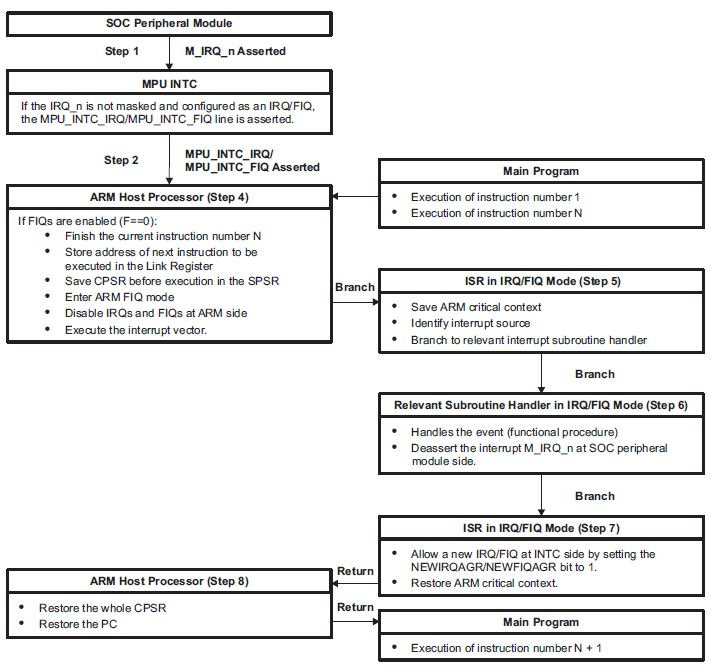
\includegraphics[scale=1]{chapters/hal/figures/interruptProcedure}
	\caption{IRQ/FIQ Verarbeitung \cite[S. 193]{ARM:TRM}}
	\label{fig:interruptProcedure}
\end{figure}

\pagebreak 